\documentclass{rapport}

\usepackage{lipsum}

\usepackage{gensymb}

\usepackage{float}

\usepackage{graphicx} % Required for inserting images

\title{file title} %title of the file

 

\begin{document}

 

%----------- Report information ---------

 

\logo{src/ua_iut_h_couleur_ecran.png}

\uni{\textbf{IUT Angers}}

\ttitle{SAé Robot - Rapport de CAO} %title of the file

\name{Saé Robot} % Project Name

\subject{SAé Robot} % Subject name

\topic{Raport de projet} % Topic name

 

\professor{Mme. Alyssia DONG \\

           M. Patrice Mangeard\\
           
}

 

\students{Charly PAYRAUDEAU} % information related to the students

 

%----------- Init -------------------

       

\buildmargins % display margins

\buildcover % create the front cover of the document

\toc % creates the table of contents

 

%------------ Report body ----------------

 

\section{Introduction}

\label{sec:introduction}

Dans le cadre de la SAE Robotique, nous avons été chargés de concevoir deux cartes mères pour un robot participant à un challenge de course. L'objectif principal était de développer des cartes électroniques capables de gérer les fonctionnalités essentielles du robot, notamment [ajouter les fonctionnalités principales]. Ce projet s'inscrit dans une démarche pédagogique et compétitive, nous permettant d'acquérir des compétences pratiques en conception assistée par ordinateur (CAO) et en électronique.

 

Pour mener à bien ce projet, nous avons utilisé le logiciel \textbf{Eagle}, un outil performant et adapté à la conception de schémas électroniques et au routage de cartes. La principale contrainte était de respecter les délais imposés par le challenge, tout en garantissant la fiabilité et l'efficacité des cartes. Ce projet représente également un défi technique, avec des exigences élevées en termes de miniaturisation, de performance, et de robustesse.

 

\section{Cahier des charges}

\label{sec:cahier_des_charges}

la carte 1 est composé d'un comparateur qui mesure avec la capteur infrarouge la distance à laquelle nous nous trouvons et envoi un signal digital à l'arduino, ensuite, les deux autres capteurs infrarouge sont reliés eux à des pins analogiques, pour avoir des valeurs de 0 à 255, pareil pour le capteur à ultra son. et pour finir le signal digital du servo moteur envoyé à un pin pwm de l'arduino.
\end{itemize}

 

Pour assurer le bon fonctionnement de cette LED bicolore, deux comparateurs sont dédiés à chacune des couleurs. Les seuils de tension des comparateurs sont ajustables à l’aide de deux potentiomètres intégrés. Par ailleurs, chaque LED, qu’elle soit unicolore ou bicolore, est reliée à une résistance de pull-up, garantissant une polarisation correcte et un fonctionnement stable.

 
\newpage
 

\section{Schéma fonctionnel de la carte}

\label{sec:schematic_functional}

\begin{figure}[h!]

    \centering

    % Incluez ici le diagramme fonctionnel.

    \includegraphics[width=0.8\textwidth]{src/Schéma_fonctionnel_carte_1.jpg}

    \caption{Schéma fonctionnel de la carte.}

    \label{fig:functional_diagram}

\end{figure}

 

\section{Schéma structurel de la carte}

\label{sec:schematic_structural}

\begin{figure}[h!]

    \centering

    % Incluez ici le schéma structurel.

    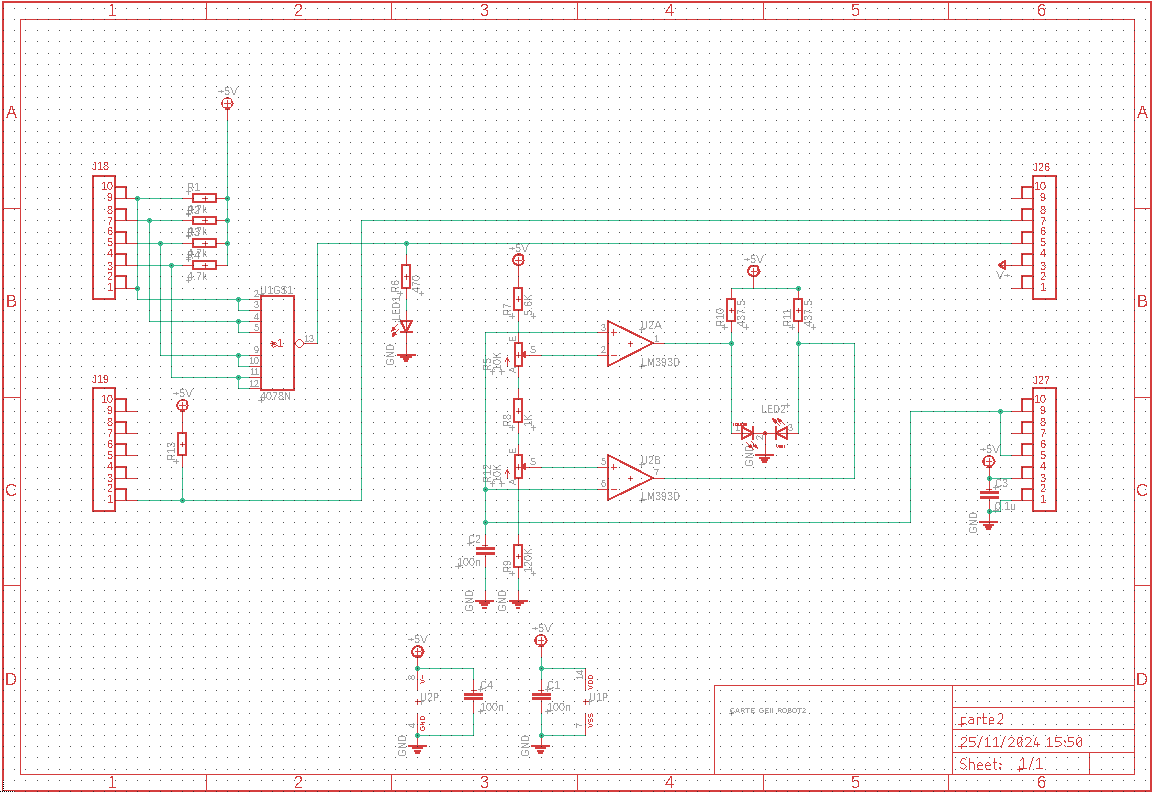
\includegraphics[width=0.8\textwidth]{src/carte.PNG}

    \caption{Schéma structurel de la carte.}

    \label{fig:structural_diagram}

\end{figure}

J'ai relier les capteurs infra rouges aux entrées analogiques de l'arduino, dont une qui est reliée à un comparateur. Celui ci me permet d'indiquer à l'arduino par un signal digital (0 ou 1) si un obstacle se trouve devant. J'allume également une led si un obstacle se trouve devant mon capteur. J'ai mis en amont du comparateur un potentiomètre de 10k Ohms et une resistance devant et derriere ce potentiomètre. Devant la led, j'ai mis une resistance de 330 Ohms, comme indiqué dans la documentation constructeur.

 

\section{Capture d'écran du routage}

\label{sec:routing}

\begin{figure}[h!]

    \centering

    % Incluez ici une capture d'écran du routage.

    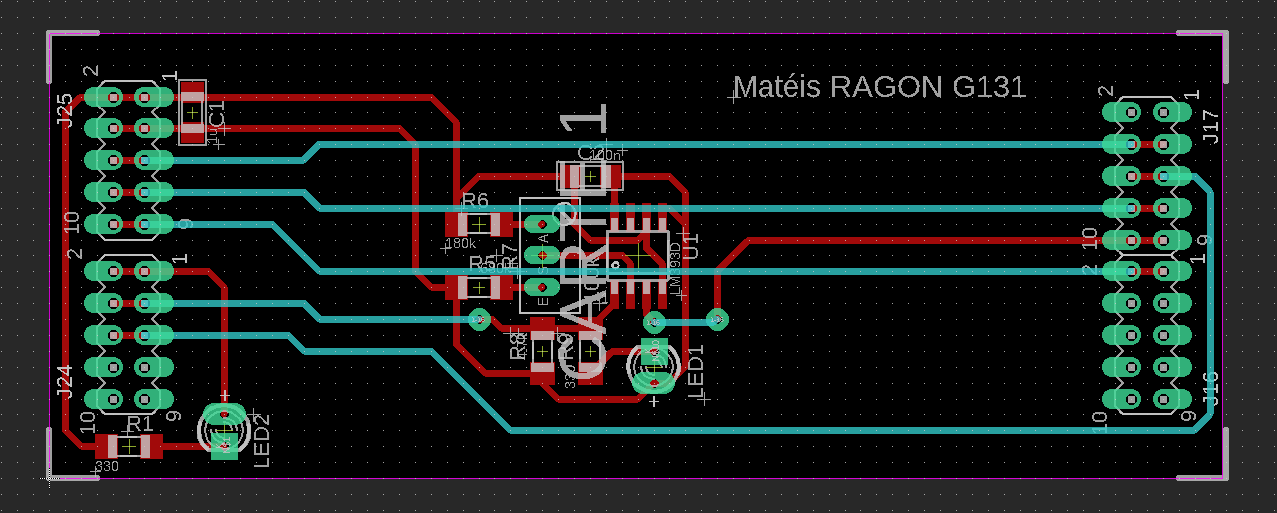
\includegraphics[width=0.8\textwidth]{src/routage.PNG}

    \caption{Capture d'écran du routage.}

    \label{fig:routing_screenshot}

\end{figure}

 

\section{Tests et mesures}

\label{sec:tests_measurements}



 

\section{Conclusion : "Et si c'était à refaire ?"}

\label{sec:conclusion}

Si c'était à refaire, je souhaiterais qu'on nous explique plus à quoi sert chaque composants, pour qu'on puisse etre en capacité de faire nos propres cartes, non pas parce que c'est comme ça qu'on les fait mais parce qu'on sait que c'est comme ça qu'on fait.

 

\section*{Annexes (facultatif)}

% Ajoutez ici toute documentation complémentaire ou données utiles.

 

\end{document}